\chapter{Rezultati}


\section{Minimizacija najvećeg odstupanja}
\quad Za genetski algoritma sa slijedećim parametrima: 
\begin{itemize}
\item vjerojatnost križanja $0,7$
\item vjerojatnost mutacije $0,02$
\item veličina populacije $100$
\item broj iteracija $50000$
\item funkcija cilja $f(\varphi)=max\left( \mid M_{konst}-M(\varphi)\mid\right) $
\end{itemize}
dobiveni su slijedeći rezultati:
\begin{itemize}
\item početne koordinate točke $A(383,46\quad 70,47)$ i točke $B(-138,45\quad  92,32)$ u mm
\item maksimalni moment od $5191,7$ Nmm te minimalni moment od $5155,7$  Nmm
\item vrijednost funkcije cilja $0,0526$
\end{itemize}

Prikaz dijagrama momenta može se vidjeti na slici \ref{fig:max_m1},a funkcije cilja na slici \ref{fig:max_f1}. Najveća apsolutna razlika u odstupanju od željene vrijednosti momenta iznosi približno $18$ Nmm što je vrlo zadovoljavajuće za ovaj mehanizam.


\begin{figure}[h!]
\center
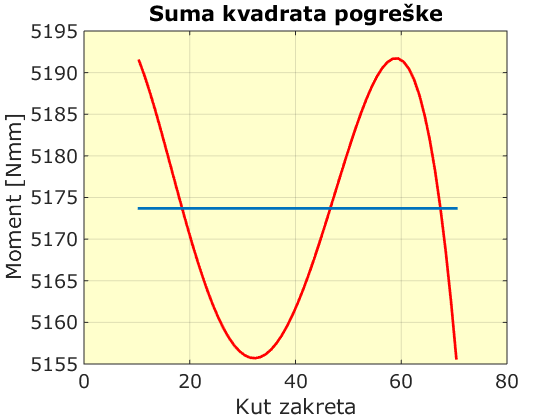
\includegraphics[scale=.6]{slike/max_m1.png}
\caption{Dijagrama odstupanja momenta od traženog (prvi set parametra)}
\label{fig:max_m1}
\end{figure}

\begin{figure}[h!]
\center
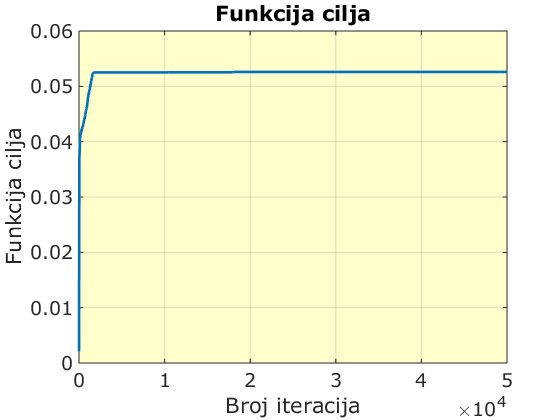
\includegraphics[scale=.6]{slike/max_f1.png}
\caption{Prikaz funkcije cilja (prvi set parametra)}
\label{fig:max_f1}
\end{figure}




\quad Drugi set parametara algoritma dan je sa slijedećim parametrima: 
\begin{itemize}
\item vjerojatnost križanja $0,7$
\item vjerojatnost mutacije $0,01$
\item veličina populacije $100$
\item broj iteracija $10000$
\item funkcija cilja $f(\varphi)=max\left( \mid M_{konst}-M(\varphi)\mid\right) $
\end{itemize}
te su dobiveni su slijedeći rezultati:
\begin{itemize}
\item početne koordinate točke $A(380,28\quad 72,63)$ i točke $B(-137,51\quad  91,57)$ u mm
\item maksimalni moment od $5192,5$  Nmm te minimalni moment od $5154,8$  Nmm
\item vrijednost funkcije cilja $0,0606$
\end{itemize}


Prikaz rezultata za drugi set parametara može se vidjeti na slikama \ref{fig:max_m2} i \ref{fig:max_f2}. Najveća apsolutna razlika u odstupanju od željene vrijednosti momenta iznosi približno $18,8$ Nmm što je vrlo zadovoljavajuće za ovaj mehanizam.

\begin{figure}[h!]
\center
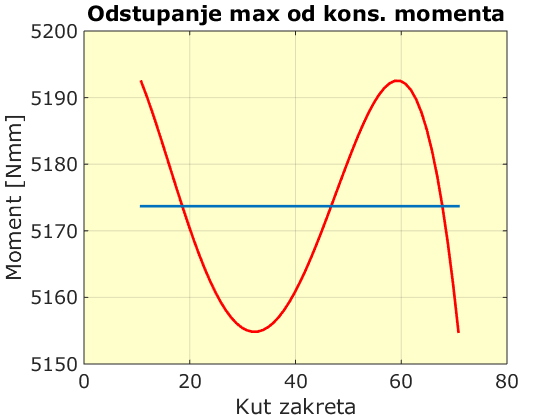
\includegraphics[scale=.6]{slike/max_m2.png}
\caption{Dijagrama odstupanja momenta od traženog (drugi set parametra)}
\label{fig:max_m2}
\end{figure}

\begin{figure}[h!]
\center
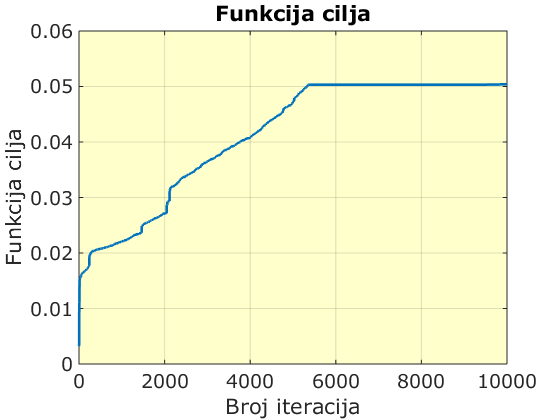
\includegraphics[scale=.6]{slike/max_f2.png}
\caption{Prikaz funkcije cilja (drugi set parametra)}
\label{fig:max_f2}
\end{figure}



\section{Suma kvadrata pogreške}

\quad Treći set parametara algoritma dan je sa slijedećim parametrima: 
\begin{itemize}
\item vjerojatnost križanja $0,7$
\item vjerojatnost mutacije $0,02$
\item veličina populacije $100$
\item broj iteracija $50000$
\item funkcija cilja $f(\varphi)=\sum_{i=1}^{n}\left( M_{konst}-M_i(\varphi) \right)$
\end{itemize}
te su dobiveni su slijedeći rezultati:
\begin{itemize}
\item početne koordinate točke $A(409,21\quad 50)$ i točke $B(-148,88\quad  99,26)$ u mm
\item maksimalni moment od $5182,9$  Nmm te minimalni moment od $5152,3$  Nmm
\item najveća apsolutna razlika u odstupanju od željene vrijednosti iznosi $21,39$ Nmm
\end{itemize}


\begin{figure}[h!]
\center
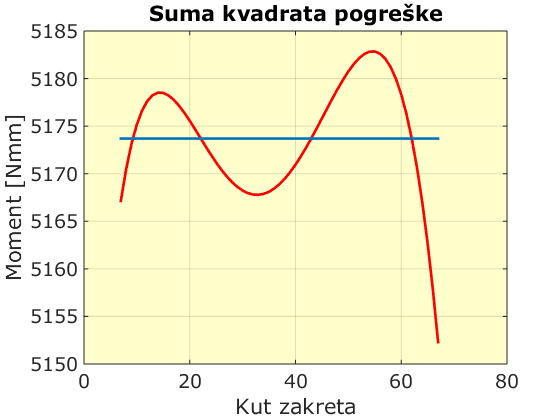
\includegraphics[scale=.6]{slike/sum_m1.png}
\caption{Dijagrama odstupanja momenta od traženog (treći set parametra)}
\label{fig:sum_m1}
\end{figure}

\begin{figure}[h!]
\center
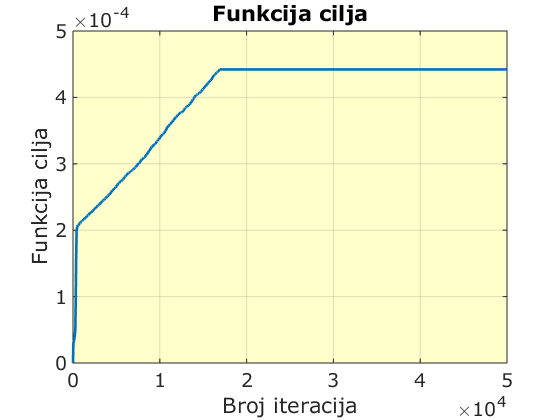
\includegraphics[scale=.6]{slike/sum_f1.png}
\caption{Prikaz funkcije cilja (treći set parametra)}
\label{fig:sum_f1}
\end{figure}



\quad Četvrti set parametara algoritma dan je sa slijedećim parametrima: 
\begin{itemize}
\item vjerojatnost križanja $0,7$
\item vjerojatnost mutacije $0,01$
\item veličina populacije $100$
\item broj iteracija $50000$
\item funkcija cilja $f(\varphi)=\sum_{i=1}^{n}\left( M_{konst}-M_i(\varphi) \right)$
\end{itemize}
te su dobiveni su slijedeći rezultati:
\begin{itemize}
\item početne koordinate točke $A(409,21\quad 50)$ i točke $B(-148,88\quad  99,26)$ u mm
\item maksimalni moment od $5182,9$ Nmm te minimalni moment od $5152,3$  Nmm
\item najveća apsolutna razlika u odstupanju od željene vrijednosti iznosi $21,38$ Nmm
\end{itemize}


\begin{figure}[h!]
\center
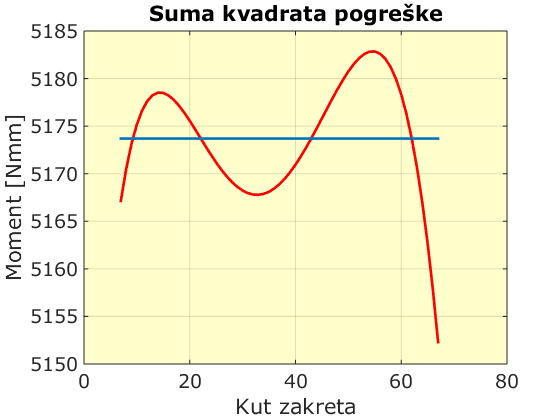
\includegraphics[scale=.6]{slike/sum_m2.png}
\caption{Dijagrama odstupanja momenta od traženog (četvrti set parametra)}
\label{fig:sum_m2}
\end{figure}

\begin{figure}[h!]
\center
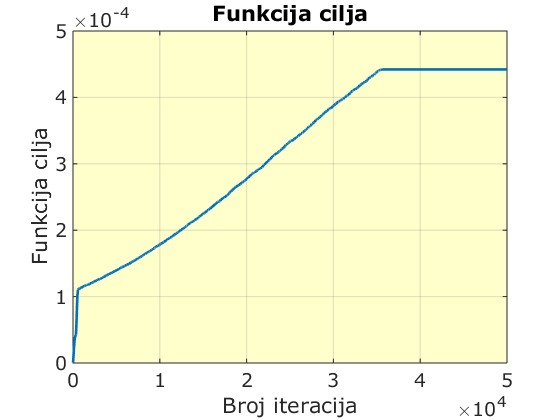
\includegraphics[scale=.6]{slike/sum_f2.png}
\caption{Prikaz funkcije cilja (četvrti set parametra)}
\label{fig:sum_f2}
\end{figure}


Sa slika \ref{fig:sum_m1} i \ref{fig:sum_m2} možemo vidjeti da momentni dijagrama za sumu kvadrata izgledaju isto i imaju iste vrijednosti. Isto tako možemo vidjeti da za vjerojatnost križanja od $0,01$ algoritmu treba puno više iteracija za konvergenciju ka točnom rješenju.


